\documentclass{standalone}
\usepackage{tikz}

\begin{document}

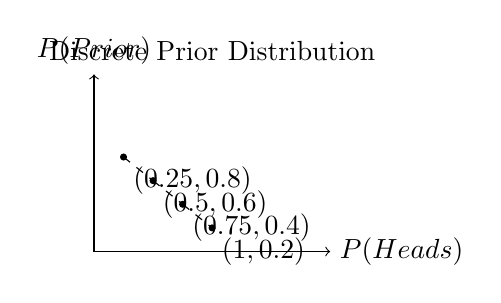
\begin{tikzpicture}[scale=1.5]
    % Define the axes
    \draw[->] (0,0) -- (2,0) node[right] {$P(\text{Heads})$};
    \draw[->] (0,0) -- (0,1.5) node[above] {$P(\text{Prior})$};

    % Draw the points representing the prior probabilities
    \fill (0.25, 0.8) circle[radius=0.03];
    \fill (0.5, 0.6) circle[radius=0.03];
    \fill (0.75, 0.4) circle[radius=0.03];
    \fill (1, 0.2) circle[radius=0.03];

    % Add labels to the points
    \node at (0.25, 0.8) [below right] {$(0.25, 0.8)$};
    \node at (0.5, 0.6) [below right] {$(0.5, 0.6)$};
    \node at (0.75, 0.4) [below right] {$(0.75, 0.4)$};
    \node at (1, 0.2) [below right] {$(1, 0.2)$};

    % Draw lines connecting the points
    \draw[dashed] (0.25, 0.8) -- (0.5, 0.6);
    \draw[dashed] (0.5, 0.6) -- (0.75, 0.4);
    \draw[dashed] (0.75, 0.4) -- (1, 0.2);

    % Title of the graph
    \node at (1, 1.7) {Discrete Prior Distribution};
\end{tikzpicture}

\end{document}